\documentclass{standalone}
\usepackage{tikz}

\usetikzlibrary{positioning,arrows}

\begin{document}
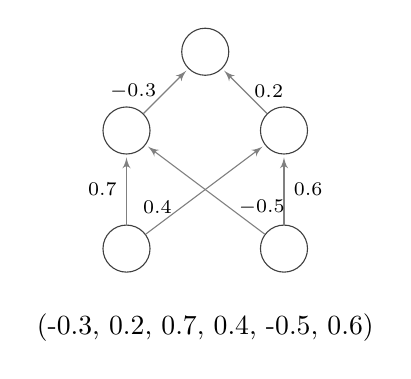
\begin{tikzpicture}[shorten >=1pt,->,draw=black!50, node distance=\layersep]
    \tikzstyle{every pin edge}=[<-,shorten <=1pt]
	\tikzstyle{neuron}=[circle,draw=black!75,minimum size=17pt,inner sep=0pt]
	\tikzstyle{input neuron}=[neuron];
	\tikzstyle{output neuron}=[neuron];
	\tikzstyle{hidden neuron}=[neuron];
	\tikzstyle{annot} = [midway, left, font=\scriptsize]
    \tikzstyle{edge} = [->, >=latex']

    \node[output neuron] (output) at (0, 2.5) {};
    \node[hidden neuron] (hiddenL) at (-1, 1.5) {};
    \node[hidden neuron] (hiddenR) at (1, 1.5) {};
    \node[input neuron] (inputL) at (-1, 0) {};
    \node[input neuron] (inputR) at (1, 0) {};

    \draw[edge] (hiddenR) edge node [annot,right] {$0.2$} (output);
    \draw[edge] (hiddenL) edge node [annot] {$-0.3$} (output);

    \draw[edge] (inputR) edge node [annot,right] {$0.6$} (hiddenR);
    \draw[edge] (inputR) edge node [annot, pos=0.3,right] {$-0.5$} (hiddenL);

    \draw[edge] (inputL) edge node [annot, left] {$0.7$} (hiddenL);
    \draw[edge] (inputL) edge node [annot, pos=0.3,left] {$0.4$} (hiddenR);

    \node (chromosome) at (0, -1) {(-0.3, 0.2, 0.7, 0.4, -0.5, 0.6)};

	%\node[input neuron, pin=left:Input \#\y] (I-\name) at (0,-\y) {};
	%node[hidden neuron] (H-\name) at (\layersep,-\y cm) {}; 
	% Draw the output layer node 
	%\node[output neuron,pin={[pin edge={->}]right:Output}, right of=H-3] (O) {}; 
	% Connect every node in the input layer with every node in the 
	% hidden layer. 
	% Connect every node in the hidden layer with the output layer 
	% Annotate the layers 
	%\node[annot,above of=H-1, node distance=1cm] (hl) {Hidden layer}; 
	%\node[annot,left of=hl] {Input layer}; 
	%\node[annot,right of=hl] {Output layer};
\end{tikzpicture}
\end{document}
